% !TEX program = xelatex
% 研究型工程文章；证据审计截止 2026-07-24。
\documentclass[UTF8,a4paper,zihao=-4,oneside]{ctexart}

\usepackage[
  top=25mm,
  bottom=25mm,
  left=30mm,
  right=25mm,
  headheight=14pt,
  footskip=12mm
]{geometry}
\usepackage{amsmath,amssymb}
\usepackage{booktabs,tabularx,array,longtable}
\usepackage{enumitem}
\usepackage{fancyhdr}
\usepackage{graphicx}
\usepackage{float}
\usepackage{xcolor}
\usepackage{listings}
\usepackage{xurl}
\usepackage{tikz}
\usetikzlibrary{arrows.meta,positioning,fit,calc}
\usepackage[hidelinks]{hyperref}

% 排版借用研究生论文常见的宋体、黑体、Times New Roman、A4 版心和三线表。
% 内容是一篇研究型工程反思，不设置封面、声明、学位信息和空白页。
\setCJKmainfont[BoldFont=SimHei]{SimSun}
\setCJKsansfont[BoldFont=SimHei]{SimHei}
\setmainfont{Times New Roman}

\setlength{\parindent}{2em}
\setlength{\parskip}{0pt}
\linespread{1.40}
\setlength{\emergencystretch}{3em}
\setlist{leftmargin=2.2em,itemsep=0.25em,topsep=0.35em}
\widowpenalty=10000
\clubpenalty=10000
\displaywidowpenalty=10000
\setcounter{secnumdepth}{3}

\ctexset{
  section={
    number=\arabic{section},
    format=\zihao{3}\heiti,
    beforeskip=2.2ex,
    afterskip=1.2ex
  },
  subsection={
    format=\zihao{4}\heiti,
    beforeskip=1.7ex,
    afterskip=0.8ex
  },
  subsubsection={
    format=\zihao{-4}\heiti,
    beforeskip=1.2ex,
    afterskip=0.5ex
  },
  paragraph={
    format=\zihao{-4}\heiti,
    beforeskip=1.0ex,
    afterskip=0.4ex,
    runin=false
  }
}

\pagestyle{fancy}
\fancyhf{}
\fancyfoot[C]{\zihao{5}\thepage}
\renewcommand{\headrulewidth}{0pt}
\renewcommand{\footrulewidth}{0pt}
\fancypagestyle{plain}{%
  \fancyhf{}
  \fancyfoot[C]{\zihao{5}\thepage}
  \renewcommand{\headrulewidth}{0pt}
}

\newcolumntype{Y}{>{\raggedright\arraybackslash}X}
\newcolumntype{C}[1]{>{\centering\arraybackslash}p{#1}}
\newcolumntype{L}[1]{>{\raggedright\arraybackslash}p{#1}}
\newcommand{\taskpath}[1]{\path{#1}}
\newcommand{\statusword}[1]{\texttt{#1}}
\newcommand{\claimstatus}[1]{\texttt{#1}}
\graphicspath{{assets/}}

\renewcommand{\lstlistingname}{代码}
\lstdefinestyle{thesiscode}{
  basicstyle=\ttfamily\zihao{-5},
  numbers=left,
  numberstyle=\ttfamily\zihao{6},
  numbersep=8pt,
  xleftmargin=2.4em,
  framexleftmargin=2.0em,
  frame=single,
  framesep=4pt,
  framerule=0.4pt,
  rulecolor=\color{black},
  columns=fullflexible,
  keepspaces=true,
  breaklines=true,
  breakatwhitespace=false,
  showstringspaces=false,
  tabsize=2,
  captionpos=t,
  aboveskip=.7em,
  belowskip=.7em
}
\lstset{style=thesiscode}

\newenvironment{evidencebox}{%
  \par\smallskip
  \begingroup\small
  \noindent\rule{\linewidth}{0.4pt}\par\smallskip
  \noindent\textbf{证据与边界：}\ignorespaces
}{%
  \par\smallskip\noindent\rule{\linewidth}{0.4pt}
  \endgroup\par\medskip
}

\newenvironment{researchclaim}{%
  \begin{quote}\small\noindent\textbf{研究判断：}\ignorespaces
}{%
  \end{quote}
}

\hypersetup{
  pdftitle={从提示约束到可执行约束：仓库级 RTL Agent 的证据闭环与声明—证据失配治理},
  pdfsubject={基于 ysyx-workbench 四月至七月工程记录的探索性研究},
  pdfkeywords={RTL Agent, 可执行约束, design-id, mutation, fail-closed, RV64}
}

\begin{document}

\thispagestyle{plain}
\begin{center}
  {\zihao{2}\heiti 从提示约束到可执行约束\par}
  \vspace{0.35em}
  {\zihao{3}\heiti 仓库级 RTL Agent 的证据闭环与声明—证据失配治理\par}
  \vspace{0.8em}
  {\zihao{-4}基于 2026 年 4—7 月工程记录的探索性研究\par}
\end{center}

\vspace{0.8em}
\noindent\textbf{摘\quad 要：}
在寄存器传输级（Register Transfer Level，RTL）工程中，人工智能 Agent
可以生成能够编译的代码，也可以调用仿真、综合和静态时序分析（Static Timing
Analysis，STA）工具。然而，“命令返回
0”“局部测试通过”或“报告中出现 PASS”都可能强于真实证据：测试可能没有覆盖目标故障，
日志可能属于旧设计，局部优化可能破坏系统回归，代理时序也可能被误写成物理签核。
本文把这种\textbf{结论强于证据允许范围}的状态称为“声明—证据失配”；为对应工程记录中的
原用语，下文亦简称“假完成”。它判断的是主张与证据的关系，不涉及实现者的主观动机。

本文以 \taskpath{ysyx-workbench} 中 2026 年 4—7 月的 task-run、原始日志、结构化结果和
回滚记录为材料，研究自然语言约束如何迁移为可执行工程约束。所分析的机制包括：
有界上下文召回、任务合同、设计身份（design-id）绑定、分层验证、负向 RTL 变体、
证据新鲜度、失败关闭发布和回滚。四个月记录显示，这些机制曾实际暴露 lint-only 的
功能空白、定向测试后的组合环、分支推测与 JALR pending 的死锁、跨设计证据错配以及
mutation oracle 的假绿风险；多个候选因此被拒绝或回退。七月的部分切片已能把
focused test、模块回归、负向变体、原始日志哈希和 full-core GAP 同时保存在一条证据链中。

这些结果支持一个有限结论：在本文所列案例中，把 Prompt 中的要求编译成机器可检查的
对象、配置、命令、反例和发布条件，为 Agent 主张的归属、检验、拒绝和限定提供了机制。
本文并未证明
反馈闭环在总体上必然优于单次 Prompt，因为模型、代码、任务和工具在纵向记录中同时变化。
为此，文末提出 B0—B3 受控实验和组件消融方案，把因果问题留给同模型、同快照、同预算的
后续研究。

\vspace{0.4em}
\noindent\textbf{关键词：}RTL Agent；可执行约束；证据闭环；design-id；mutation；
失败关闭；RV64

\section{引言：从“能生成”到“能被工程接受”}

四月时，我主要把 AI 当作代码生成器。它可以一次铺开若干 RTL 模块，Verilator
也能完成 lint；但如果没有 testbench、镜像加载、对拍和退出状态，所谓“完成”只能说明
语法进入了下一阶段。五月以后，AI 开始跨越 Cache、乱序后端和 SoC 修改多个文件，
候选生成速度上升，错误半径也随之扩大。六月和七月，真正改变交付质量的工作不再只是
换模型或写更多 Prompt，而是持续改造工程环境：让 Agent 知道应读取哪些事实、如何运行
真实工具、结果属于哪份设计、什么反例必须出现，以及证据不足时为什么不能宣布完成。

这段经历使我逐渐形成一个判断：

\begin{researchclaim}
模型能力影响候选生成的范围；工程环境则为这些候选能否被验证、拒绝和安全采用提供条件。
工程师为 Agent 构造的可观察性、身份、反馈和发布制度，本身就是智能工程系统的一部分。
\end{researchclaim}

这个判断不能靠“后来的任务更复杂、Token 更多、PASS 数更多”来证明。表
\ref{tab:intro-conflicts}列出三个真实冲突：每个冲突都说明，工程结论必须比工具输出多一层
语义约束。

\begin{table}[htbp]
  \centering
  \small
  \caption{工具结果与工程结论之间的典型断层}
  \label{tab:intro-conflicts}
  \begin{tabularx}{\linewidth}{@{}L{0.22\linewidth}YY@{}}
    \toprule
    表面结果 & 真实记录 & 能够成立的结论 \\
    \midrule
    9 个 RTL 文件且 lint 通过 &
    四月 RV32I 尚无 testbench、镜像加载和 NEMU 对拍 &
    语法和部分结构进入可仿真前状态，功能仍未知 \\
    focused test 通过 &
    五月 branch+ret 候选随后出现 \texttt{UNOPTFLAT}；六月分支推测破坏系统回归 &
    定向测试只证明局部场景，不能替代结构与聚合门禁 \\
    5 ns 下最差裕量为正 &
    仍有 303 个输入、1873 个输出缺少 delay，1875 个 endpoint 未约束 &
    只是在给定代理约束下通过内部路径筛选，不是物理签核 \\
    \bottomrule
  \end{tabularx}
\end{table}

本文将“声明—证据失配”（简称“假完成”）定义为：
\textbf{Agent 或流程给出的完成声明，强于该设计身份、配置、
验证层级和反例能力实际支持的范围。}它不要求代码一定错误；只要证据不足以支持声明，
就已经构成交付风险。

本文的三项主要贡献如下。

\begin{enumerate}
  \item 提出\textbf{可执行约束迁移}框架：把“基于当前设计”“验证通过”“性能更优”
  和“任务完成”等自然语言要求，拆成设计对象、配置、命令、返回码、负向证据、
  发布条件和主张边界。
  \item 把 bounded recall、task contract、design-id、mutation、分层回归、freshness、
  失败关闭和 rollback 组织成仓库级证据闭环，并用真实 RV64 案例说明其数据流。
  \item 建立主张—证据映射和只读复核入口，区分
  \claimstatus{SUPPORTED}、\claimstatus{PARTIALLY\_SUPPORTED}、
  \claimstatus{OBSERVATIONAL\_ONLY}、\claimstatus{CONTRADICTED} 与
  \claimstatus{MISSING}，避免以 PASS 数替代论证。
\end{enumerate}

本文不作三项强主张：不证明 Loop 必然优于 Prompt；不把 task-run 或 Token 数解释为
生产率；不把 Yosys 通用结构和代理 STA 写成目标工艺的物理 PPA 结论。

\section{研究问题与概念边界}

\subsection{研究问题}

\begin{table}[H]
  \centering
  \small
  \caption{研究问题及当前可回答范围}
  \label{tab:rqs}
  \begin{tabularx}{\linewidth}{@{}C{0.08\linewidth}Y L{0.24\linewidth}@{}}
    \toprule
    编号 & 问题 & 当前证据属性 \\
    \midrule
    RQ1 &
    自然语言约束能够在多大程度上迁移为可执行工程约束？ &
    工具行为与案例可观察；总体因果效应缺失 \\
    RQ2 &
    design-id、哈希、freshness 和原子发布能够关闭哪些证据错配路径？ &
    已有身份错配和重放案例；系统化故障注入不足 \\
    RQ3 &
    mutation-qualified verification 能在多大程度上证明验证环境具有故障辨识能力？ &
    对指定非等价 fault set 成立，不外推全部故障 \\
    RQ4 &
    反馈、分层门禁和回滚如何影响 RTL 搜索中候选的接受与拒绝？ &
    多个真实回滚事件；相对单 Prompt 的平均收益未知 \\
    \bottomrule
  \end{tabularx}
\end{table}

\subsection{术语解释}

\begin{table}[H]
  \centering
  \small
  \caption{本文使用的核心术语（1）}
  \label{tab:terms}
  \begin{tabularx}{\linewidth}{@{}L{0.20\linewidth}L{0.32\linewidth}Y@{}}
  \toprule
  术语 & 通俗含义 & 在本文中的严格作用 \\
  \midrule
  Prompt 约束 &
  用自然语言告诉模型“应该做什么” &
  便于表达意图，但不自动提供对象身份、执行命令、失败条件和证据边界 \\
  可执行约束 &
  能由脚本、测试或验证器判定的条件 &
  例如指定 design-id、命令返回码、测试分子/分母、唯一失败 marker 和晋级
  （promotion，即允许候选进入下一交付状态）门 \\
  task-run &
  一次工作流活动留下的目录 &
  保存上下文、调度、日志、报告和证据；目录数不是独立实验数 \\
  bounded recall &
  有大小和范围上限的上下文召回 &
  在 canonical 规则、profile 和独立任务焦点之间分配上下文，缺焦点时失败关闭 \\
  task contract &
  任务开始前冻结的输入、输出、动作和成功条件 &
  防止执行过程中悄悄改变验收标准 \\
  design-id &
  当前 RTL 文件集合内容的数字身份 &
  证明“证据属于哪份设计”，不证明该设计正确 \\
  \bottomrule
  \end{tabularx}
\end{table}

\begin{table}[H]
  \centering
  \small
  \caption{本文使用的核心术语（2）}
  \label{tab:terms-cont}
  \begin{tabularx}{\linewidth}{@{}L{0.20\linewidth}L{0.32\linewidth}Y@{}}
  \toprule
  术语 & 通俗含义 & 在本文中的严格作用 \\
  \midrule
  oracle &
  判断结果正确或错误的观测规则 &
  testbench、断言、差分模型和日志解析器都可能是 oracle，也可能有盲点 \\
  mutation &
  有意构造一份包含指定错误的可编译 RTL 变体 &
  用于检验 oracle 能否拒绝已知错误，不等价于穷尽全部故障 \\
  freshness &
  证据是否晚于并绑定当前语义输入 &
  不能用 \texttt{touch} 把旧内容伪装成新证据 \\
  fail-closed &
  身份、证据或配置有疑问时拒绝完成 &
  局部 PASS 不足时保留 \texttt{GAP} 或 \texttt{UNQUALIFIED} \\
  rollback &
  候选违反门禁后恢复到已知设计身份 &
  回退后仍需重跑规定的验证，不能只说“代码已经改回去” \\
  PPA proxy &
  在简化库和约束下测量性能、功耗或面积的代理 &
  用于相对筛选；没有寄生参数交换格式（SPEF）、时钟树综合（CTS）、工艺波动分析
  （OCV）和完整 I/O 约束时，不是物理签核（signoff） \\
  \bottomrule
  \end{tabularx}
\end{table}

\subsection{失败模式}

本文把仓库中出现的风险归纳为八类，见表\ref{tab:failure-classes}。分类的目的不是制造
一个漂亮框架，而是让每一种“完成”都有相应的反例入口。

\begin{table}[htbp]
  \centering
  \small
  \caption{假完成的八类路径}
  \label{tab:failure-classes}
  \begin{tabularx}{\linewidth}{@{}C{0.07\linewidth}L{0.31\linewidth}YY@{}}
    \toprule
    类别 & 失败路径 & 仓库反例 & 对应约束 \\
    \midrule
    A & 语法通过冒充功能正确 & 四月 RV32I 只有 lint & 动态 TB、镜像与对拍 \\
    B & 局部通过冒充系统通过 & focused PASS 后组合环或聚合失败 & 分层回归 \\
    C & 代理指标冒充签核 & generic cells、理想时钟 STA & PPA 资格边界 \\
    D & 不可比指标拼成趋势 & 不同 workload 的 CPI & matched configuration \\
    E & 过期或跨设计证据 & live design 与 candidate 不同 & design-id/source-id \\
    F & 不完整材料被发布 & marker、publication、DB 不一致 & 原子发布与 strict guard \\
    G & 弱 oracle 造成假绿 & 同值连接、旧值 force/release & 非对称刺激与变体身份 \\
    H & 搜索失败未回滚 & 双 memory 退化、分支推测活锁 & rollback 与重验证 \\
    \bottomrule
  \end{tabularx}
\end{table}

\section{仓库级 RTL Agent 的系统设计}

\subsection{总体闭环}

图\ref{fig:system-loop}给出当前系统的主数据流。这里最重要的不是方框数量，而是每个箭头
都传递明确对象：需求进入上下文与任务合同；候选进入真实工具；工具输出进入证据层；
证据层决定接受、拒绝或回滚；只有已验证事实才进入下一轮有界召回。

\begin{figure}[htbp]
  \centering
  \resizebox{0.98\linewidth}{!}{%
  \begin{tikzpicture}[
    box/.style={draw=black,rounded corners=1pt,align=center,
      text width=25mm,minimum height=11mm,inner sep=4pt,font=\small},
    wide/.style={box,text width=32mm},
    flow/.style={-{Latex[length=2.1mm]},thick},
    back/.style={-{Latex[length=2.1mm]},thick,dashed}
  ]
    \node[box] (goal) {用户目标\\与风险边界};
    \node[wide,right=6mm of goal] (recall) {bounded recall\\canonical / profile\\ / focus};
    \node[box,right=6mm of recall] (contract) {task contract\\对象/动作/成功条件};
    \node[box,right=6mm of contract] (agent) {Agent\\生成候选};
    \node[wide,below=9mm of agent] (layer) {分层验证\\focused→module\\→system→PPA};
    \node[wide,left=6mm of layer] (negative) {mutation / 反例\\oracle 辨识能力};
    \node[wide,left=6mm of negative] (identity) {design-id / hashes\\freshness /\\configuration};
    \node[wide,left=6mm of identity] (publish) {fail-closed publication\\接受 / GAP / rollback};
    \draw[flow] (goal) -- (recall);
    \draw[flow] (recall) -- (contract);
    \draw[flow] (contract) -- (agent);
    \draw[flow] (agent) -- (layer);
    \draw[flow] (layer) -- (negative);
    \draw[flow] (negative) -- (identity);
    \draw[flow] (identity) -- (publish);
    \draw[back] (publish.north) to[out=135,in=225] (recall.south);
    \draw[back] (publish.south) to[out=-25,in=-155] (agent.south);
  \end{tikzpicture}}
  \caption{从自然语言需求到可消费证据的闭环}
  \label{fig:system-loop}
\end{figure}

一次执行同时包含三条流：

\begin{itemize}
  \item \textbf{控制流}决定下一步执行什么、失败后是否停止；
  \item \textbf{工程数据流}承载源码、配置、仿真输入和 EDA 输出；
  \item \textbf{证据流}把原始日志、身份、哈希、状态和结论边界连接起来。
\end{itemize}

仿真返回 0 只属于工程数据流。只有结果被绑定到当前设计、负向验证具有辨识力、
上层门禁没有失败，证据流才允许它成为交付结论。

\subsection{有界上下文与任务合同}

对一个大型仓库，Agent 不是“读得越多越好”。无界历史会把过期结论、旧路径和相互冲突的
设计状态带入上下文。当前环境把上下文分成 canonical 规则、任务 profile 和独立
non-history focus。若焦点不能由独立材料支持，召回失败，而不是用同一 task-run 自证。

任务合同进一步冻结：

\[
\text{Contract} =
\{\text{objects},\text{inputs},\text{actions},\text{outputs},
\text{success},\text{forbidden extrapolation}\}.
\]

这使“完成 FENCE”不再是一个抽象目标，而会被拆成具体 RTL module/signal/transaction、
规定的 testbench、负向变体、原始日志和 full-core 边界。合同本身仍可能写错，因此它是
可审查输入，不是正确性的来源。

\subsection{profile 如何变成可执行节点}

profile 文件虽然使用 \texttt{.tsv} 后缀，实际按竖线分为六列：

\begin{center}
\texttt{node | module | function | owner | inputs | outputs}
\end{center}

代码\ref{code:profile-loader}来自 \taskpath{scripts/agent-e2e.sh}。它说明
\texttt{@include} 不是一个执行节点，而是递归展开另一个 profile。

\begin{lstlisting}[language=bash,firstnumber=180,
  caption={profile 递归展开的实际加载逻辑},
  label={code:profile-loader}]
while IFS= read -r line || [[ -n $line ]]; do
  [[ -z $line ]] && continue
  [[ $line = \#* ]] && continue
  IFS='|' read -r node module function owner inputs outputs <<< "$line"
  if [[ $node = "@include" ]]; then
    load_profile "$module"
    continue
  fi
  PROFILE_NODE_IDS+=("$node")
  PROFILE_MODULES+=("$module")
  PROFILE_FUNCTIONS+=("$function")
  PROFILE_OWNERS+=("$owner")
  PROFILE_INPUTS+=("$inputs")
  PROFILE_OUTPUTS+=("$outputs")
  PROFILE_SOURCES+=("$profile")
done <<< "$profile_content"
\end{lstlisting}

逐行看，这段代码完成五件事：跳过空行和注释；按六列拆分；递归展开 include；保存每个
节点的函数与责任；记录节点来自哪个 profile。于是，一个表面只有八行的
\taskpath{agent-system.tsv}，因为包含 discovery，最终形成十节点 closure。后续 report、
manifest、dispatch、\taskpath{nodes.tsv} 和 evidence index 都必须与这个 closure 同序。
这不是为了让配置更复杂，而是防止“文档写了一个流程，实际执行了另一个流程”。

\subsection{设计身份：证明证据属于谁}

design-id 是 canonical RTL 文件集合的 SHA-256。代码\ref{code:design-id}来自
\taskpath{npc/rv64/eval/ppa/tools/fence_ordering_evidence.py}。它先计算 RTL 绑定，
再用同一身份解析程序日志、focused 日志和模块聚合。

\begin{lstlisting}[language=Python,firstnumber=343,
  caption={FENCE 证据构建器中的 design-id 绑定},
  label={code:design-id}]
rtl_sha, rtl_files = arch.rtl_binding(root)
design_id = f"sha256:{rtl_sha}"
metrics = parse_program_log(program_log, design_id)
focused_logs = {
    "program": program_log,
    "drain_gate": drain_gate_log,
}
focused = parse_focused_logs(focused_logs, design_id)
module_aggregate = parse_module_aggregate(
    root, module_summary, design_id)
variants = validate_variants(root, variant_summary)
\end{lstlisting}

如果当前工作树从 \texttt{2eff...} 变为 \texttt{08d3...}，旧测试即使内容看起来仍然
“全绿”，也不能自动成为新设计的证据。design-id 解决的是归属问题，不是正确性问题：
同一身份下仍可能有未覆盖 bug；但没有身份时，连“测试的是哪份设计”都无法回答。

\subsection{mutation-qualified verification}

正向测试回答“当前设计是否通过这些输入”，负向变体回答“验证环境能否拒绝一个已知错误”。
代码\ref{code:mutation}展示 FENCE runner 的三个最低条件：替换锚点必须唯一；旧值和新值
不能相同；原版与变体的 SHA 不得相等。

\begin{lstlisting}[language=Python,firstnumber=93,
  caption={负向 RTL 变体的非空性检查},
  label={code:mutation}]
text = source.read_text(encoding="utf-8")
if text.count(spec.old) != 1 or spec.old == spec.new:
    raise ValueError(f"{spec.name}: live RTL anchor is not unique")
variant_text = text.replace(spec.old, spec.new, 1)

original_sha = sha256_bytes(text.encode("utf-8"))
variant_sha = sha256_bytes(variant_text.encode("utf-8"))
if original_sha == variant_sha:
    raise ValueError(
        f"{spec.name}: reconstructed RTL variant is a no-op")
\end{lstlisting}

这仍不够。一个变体可能实际改变了字节，却没有在当前刺激下被触发；也可能发生错误，
但传播不到观测点。仓库记录已经出现过两类典型假绿：连接 mutation 的两端在该轨迹中数值
相同；\texttt{force/release} 使用旧值，使检查没有制造真实不对称。因而本文只把同时满足
“源码改变、错误触发、错误传播、目标 oracle 拒绝、正确设计通过”的变体计入有效分母。

\subsection{分层验证与安全搜索}

当前搜索按风险逐层扩大：

\[
\begin{aligned}
\text{focused}
&\rightarrow \text{module aggregate}
\rightarrow \text{official/AM/DiffTest}\\
&\rightarrow \text{benchmark}
\rightarrow \text{synthesis/STA proxy}.
\end{aligned}
\]

低层测试提供快速反馈，高层测试控制局部优化的外溢风险。它们不是谁替代谁：focused
能够精确定位条件，系统回归能够发现跨模块耦合；PPA 只能在功能与架构门通过后比较。

候选的状态转换可写为：

\[
S_{i+1}=
\begin{cases}
\operatorname{accept}(C_i), & \text{所有必需门通过};\\
\operatorname{refine}(C_i,E_i), & \text{失败可定位且仍值得修复};\\
\operatorname{rollback}(B), & \text{候选违反硬门或方向被证伪}.
\end{cases}
\]

这里 \(C_i\) 是候选，\(E_i\) 是本轮真实反馈，\(B\) 是已知基线。五月双 memory 候选、
branch+ret 组合环和六月分支推测活锁都进入了第三个分支。

\subsection{失败关闭与原子发布}

publication 不是把“PASS”写进 Markdown。当前实现要求七个关键产物的哈希进入
\texttt{complete.marker}：\texttt{task-report.md}、\texttt{run-manifest.json}、
\texttt{context-brief.md}、\texttt{profile-resolve.md}、\texttt{evidence-index.md}、
\texttt{dispatch-log.md} 和 \texttt{nodes.tsv}；随后再检查 report、manifest、
publication 和数据库暂存集合。
代码\ref{code:publication}摘自
\taskpath{scripts/dev_memory/maintenance.py}。

\begin{lstlisting}[language=Python,firstnumber=1868,
  caption={发布事务中的二次读取与原子提交},
  label={code:publication}]
conn.execute("BEGIN IMMEDIATE")
for name, raw in snapshot.items():
    if read_ordinary(name) != raw:
        raise ValueError(
            f"artifact changed during publication: {name}")

if stored != staged_markdown:
    raise ValueError(
        "staged DB Markdown set or content changed before publication")

upsert_stored_document(conn, item, has_fts5, now)
upsert_file(conn, item, has_fts5, now)

for name, raw in snapshot.items():
    if read_ordinary(name) != raw:
        raise ValueError(
            f"artifact changed during publication commit: {name}")
conn.commit()
\end{lstlisting}

\texttt{BEGIN IMMEDIATE} 取得写事务；事务前后两次读取防止发布过程中产物被替换；DB 暂存集
必须与现场 Markdown 精确一致；任何异常触发 rollback。即便如此，本文仍不把“原子发布”
写成已覆盖所有崩溃与并发故障，因为当前纵向证据缺少完整故障注入矩阵。它已经是一项明确的
风险控制机制，其总体故障覆盖仍是 RQ2 的开放问题。

\section{研究方法与证据体系}

\subsection{数据来源和分析单位}

本文优先使用原始工具日志，其次是绑定身份的结构化结果，再次是 task-report 和 DB 摘要。
同一事实在报告和原始日志中冲突时，以原始日志和可重算身份为准。

只读脚本 \taskpath{docs/research-paper/scripts/paper_evidence_extract.py} 对四个月顶层目录
进行了盘点，见表\ref{tab:run-counts}。

\begin{table}[htbp]
  \centering
  \small
  \caption{task-run 顶层目录盘点（审计日：2026-07-24）}
  \label{tab:run-counts}
  \begin{tabular}{@{}lrrrrrrr@{}}
    \toprule
    月份 & 事件目录 & task-report & manifest & evidence index & marker & publication \\
    \midrule
    4 月 & 8 & 8 & 0 & 0 & 0 & 0 \\
    5 月 & 137 & 132 & 0 & 0 & 0 & 0 \\
    6 月 & 1246 & 1149 & 556 & 667 & 0 & 0 \\
    7 月 & 586 & 557 & 421 & 514 & 195 & 190 \\
    \bottomrule
  \end{tabular}
\end{table}

这里的“事件目录”不是独立任务、成功任务或实验样本。六月的 1246 说明记录和工作流节点
迅速增多，不能写成“完成了 1246 项工程任务”。本文的分析单位是\textbf{有明确目标、候选、
门禁和结果边界的 task episode}，一个 episode 可以包含多个目录。

\subsection{主张—证据映射}

每条主张都记录：研究轴、状态、日期、run-id、source path、raw evidence path、
design-id、配置、命令、退出码、指标、负向证据、回滚、结论边界和复现方式。完整表位于：

\begin{center}
\taskpath{docs/research-paper/claim-evidence-map.tsv}
\end{center}

当前 21 条主张中，11 条为 \claimstatus{SUPPORTED}，3 条为
\claimstatus{PARTIALLY\_SUPPORTED}，1 条为
\claimstatus{OBSERVATIONAL\_ONLY}，5 条为
\claimstatus{CONTRADICTED}，1 条为 \claimstatus{MISSING}。这些数量只是审计分类，
不是系统成绩。

\subsection{因果边界}

四月至七月并不是一个受控实验。至少有五个混杂变量同时变化：

\begin{enumerate}
  \item 模型与执行端变化；
  \item 代码规模和成熟度变化；
  \item 任务从局部 RTL 发展到跨模块、Linux 与 PPA；
  \item 工具、测试和日志能力变化；
  \item 我本人对架构、验证和 Agent 编排的理解变化。
\end{enumerate}

因此，本文能说“该门禁在这次事件中拒绝了这个候选”，不能说“相同任务下，闭环平均使
正确率提高了多少”。后者需要固定其余变量，只改变工作流条件。

\section{纵向案例：约束是如何长出来的}

\subsection{4 月：从代码生成到最小可观察闭环}

4 月 13 日的 RV32I 非流水线核心一次生成了 9 个 RTL 文件，目标包括译码、立即数、
ALU、比较、LSU、WBU 和顶层多周期状态机。Verilator lint 通过，但报告同时明确：
尚无 testbench、镜像加载器和 NEMU 对拍，普通异常仍是 halt-only。这条记录的价值不在
“AI 写了九个文件”，而在它留下了一个清楚的能力边界：代码生成速度已经高于验证能力。

随后 NPC 的 DPI/C++、AM image、pmem 和退出协议被接通，
\taskpath{hello-riscv32-npc.bin} 可以输出并以 code 0 退出；itrace、mtrace 和 dtrace
分别记录指令、内存和设备活动，batch mode 使相同输入能够无人值守重放。

\begin{evidencebox}
\taskpath{2026-04-13-rv32i-nonpipe-core} 支持“9 个 RTL 文件和 lint 通过”，也明确记录
“无 testbench、镜像和对拍”。\taskpath{2026-04-13-npc-dpic-bringup} 支持 hello 与
退出码。它们共同证明最小反馈链形成，不证明处理器已经完整正确。
\end{evidencebox}

这一阶段 AI 对工程的介入仍然较浅：我决定接口、测试和结果含义，AI 主要展开实现。
但环境开始改变角色分工——模型不再只能听我转述错误，而能看到真实程序如何执行和退出。

\subsection{5 月：候选生成变快，拒绝机制开始重要}

5 月的工作进入 Cache、SoC 和乱序后端。乱序执行要求指令在操作数就绪时选择执行，
同时由 ROB（Reorder Buffer，重排序缓冲区）保持按程序顺序退休；IQ（Issue Queue，
发射队列）保存等待执行的微操作。

5 月 29 日的记录定位了一个具体错误：ready 的新指令可以走 dispatch-bypass 直接发射，
旧 compact 逻辑却把这次发射误当作 IQ slot0 发射，删除了仍在等待操作数的 entry。
修复后，AM \texttt{add} 在该配置中得到 541 cycles / 839 commits / CPI 0.645。

更重要的是，同一 task episode 记录了两个被拒候选：

\begin{table}[htbp]
  \centering
  \small
  \caption{5 月候选的接受与拒绝}
  \label{tab:may-candidates}
  \begin{tabularx}{\linewidth}{@{}L{0.24\linewidth}Y L{0.21\linewidth}@{}}
    \toprule
    候选 & 观测 & 决策 \\
    \midrule
    IQ compact 修复 &
    定向回归通过，AM \texttt{add} 为 CPI 0.645 &
    保留 \\
    双 memory issue/buffer 放宽 &
    IQ 修复后可 GOOD TRAP，但 CPI 从 0.645 退化到 0.665 &
    回退到单 memory 策略 \\
    lane0 branch + lane1 ret &
    focused test 通过，完整 build 出现 \texttt{UNOPTFLAT} 组合环 &
    回退 \\
    \bottomrule
  \end{tabularx}
\end{table}

这说明 Agent 已经能够产生多个架构候选，但真正构成工程能力的是环境能否对候选说“不”。
CPI 只在同一程序、编译选项和测量边界内可比；5 月其他记录中的 CoreMark phase metric
不能与 0.645 直接拼成趋势线。

\subsection{6 月：跨模块任务暴露了局部正确性的极限}

六月开始形成 profile、manifest、bounded recall 和实现者/审查者分离。AI 可以在更长的
任务链中阅读多个模块，但也更容易把一个局部组件的通过误写成系统方案成立。

分支推测案例最能说明这个问题。把休眠 checkpoint 路径从
\texttt{1'b0} 打开后，lint 和 module 113/113 通过；系统回归却变为 riscv-tests
255/16、AM 25/32。回退后恢复 271/0 和 113/113。随后 ROB-walk 恢复 FSM、rename restore
和 IQ squash 分别通过隔离测试，整合打开后仍得到 riscv-tests 251/20、AM 14/43。

trace 最终把问题定位到协议耦合，而非 ROB-walk 本身：branch speculation active 时
commit 被冻结，JALR 仍进入 pending 并等待后端 drain；drain 需要 ROB 排空，ROB 又需要
commit，形成闭环等待。局部恢复组件正确，并不能修复前端推测与 jump pending 的整体协议。

\begin{lstlisting}[language={},numbers=none,
  caption={分支推测 task-run 中的关键验证结果}]
spec-on checkpoint: riscv-tests 255/16, AM 25/32
rollback mode=0:    riscv-tests 271/0,  module 113/113
ROB-walk spec-on:   riscv-tests 251/20, AM 14/43
root cause: branch-spec active <-> pending JALR drain deadlock
\end{lstlisting}

\begin{evidencebox}
数据来自 \taskpath{.github/task-runs/2026-06-29-rv64-ooo-core-architecture-constitution/report.md}。
它支持“聚合门禁发现并回退了该候选”，不支持“ROB-walk 无效”或“所有分支推测方案都会失败”。
\end{evidencebox}

\subsubsection{Ubuntu 里程碑：同一个词必须有不同证据等级}

NEMU 与 NPC 的 Ubuntu 日志也是一次结论边界训练。NEMU 的原始 console 记录了：

\begin{lstlisting}[language={},numbers=none,
  caption={NEMU 挂载 Ubuntu rootfs 并进入 shell 的日志摘录}]
virtio_blk virtio0: [vda] 4194304 512-byte logical blocks
VFS: Mounted root (ext4 filesystem) on device 254:0.
PRETTY_NAME="Ubuntu 22.04.5 LTS"
[ysyx-rootfs-sh] /bin/sh -c marker
[ysyx-rootfs] /bin/sh -c exit=0
[ysyx-rootfs] launching /bin/sh
/bin/sh: 0: can't access tty; job control turned off
\end{lstlisting}

NPC 的对应 console 则到达：

\begin{lstlisting}[language={},numbers=none,
  caption={NPC rootfs mount 与 systemd/banner 里程碑日志摘录}]
virtio_blk virtio0: [vda] 4194304 512-byte logical blocks
VFS: Mounted root (ext4 filesystem) on device 254:0.
systemd[1]: systemd 249.11-0ubuntu3.21 running in system mode
systemd[1]: Hostname set to <ysyx-ubuntu2204>.
\end{lstlisting}

NEMU 可以写“进入 \texttt{/bin/sh}”；NPC 只能写“rootfs mount + systemd/banner smoke”。
NPC 报告明确没有真实 root prompt，也没有
\texttt{\_\_NPC\_SYSTEMD\_CHECK\_DONE\_\_ rc=0}。里程碑并没有因此失去价值；恰恰是
保留 GAP，使后来者知道下一步还差什么。

\subsection{7 月：让证据本身也接受验证}

\subsubsection{Yosys：结构成功不等于 PPA 成功}

7 月 15 日的一次轻量 Yosys 日志给出：

\begin{lstlisting}[language={},numbers=none,
  caption={R3P4 light-Yosys 结构统计摘录}]
18115 wires
296118 wire bits
14645 cells
  507  $dff
 6768  $mux
 1568  $pmux
Warnings: 76 unique messages, 124 total
End of script. ... time: 24.82s
\end{lstlisting}

这些数字证明指定输入成功进入通用结构展开，也帮助识别 mux 和状态规模；它们不带目标工艺
面积单位，也没有证明 STA、布局布线或功耗。因此，“Yosys 仿真”在严谨表述中应改为
“Yosys 综合/结构审计”，generic cell 不能被直接写成物理面积。

\subsubsection{从正向 PASS 到故障辨识}

取指单元（Instruction Fetch Unit，IFU）的 V9I 切片在 design-id \texttt{6236...} 下得到
focused 4/4、module 109/109，并让 19 个
compile-success 负向 RTL 变体被动态拒绝。FENCE V9M 在 \texttt{2eff...} 下得到
focused 2/2、module 109/109、变体 2/2、validator 12/12。STORE/AMO V9N 又增加跨
非阻塞赋值（Non-Blocking Assignment，NBA）结算边沿的事务所有权驻留检查器，
两份源码变体均被拒绝。这里 STORE 是存储指令，AMO 是原子内存操作
（Atomic Memory Operation）。

这些数字的价值不在“PASS 更多”，而在验证环境必须表现出区分能力。例如，FENCE 的两个
负向变体分别破坏 drain gate 中的 memory-idle 条件，以及
CoreGlue 到 ControlPlane 的 \texttt{mem\_idle} 连接。只有目标 testbench 唯一报错、
正向设计通过、production source 前后 SHA 不变，才能把这次 mutation 计为有效。

\subsubsection{单模块三快照演化：从“后端排空”到 FENCE 专用内存静默}

为了避免只列举“做过什么”，本文选择
\taskpath{npc/rv64/vsrc/control/OooPendingDrainResolveGate.v} 作为纵向剖面。
该模块把 ROB、发射队列、待处理控制事件和内存静默条件归约为
\texttt{drain\_complete\_o}。这里的 drain 不是清空或复位，而是停止接纳会破坏顺序的新工作，
同时允许已经发出的不可撤回事务走到终结响应。表\ref{tab:drain-evolution}中的三个快照均由
不可变 Git 提交和文件 SHA-256 标识；短哈希只用于排版，完整值保存在
\taskpath{docs/research-paper/module-evolution-evidence.md}。

\begin{table}[htbp]
  \centering
  \footnotesize
  \caption{\texttt{OooPendingDrainResolveGate} 的三快照源码与证据边界}
  \label{tab:drain-evolution}
  \begin{tabularx}{\linewidth}{@{}C{0.10\linewidth}L{0.19\linewidth}YL{0.29\linewidth}@{}}
    \toprule
    快照 & 源码身份 & 可观察的合同差异 & 当时能够支持的证据 \\
    \midrule
    A：6 月 28 日 &
    commit \texttt{0bb371593}；文件 \texttt{e0ac...8c7} &
    ROB、IQ、退休计数与 synthetic pending 共同定义后端排空；尚无显式存储侧静默输入 &
    同一文件字节延续到战役终点；战役级 module 112/112、official 271/0、
    AM 56/56，但没有为该谓词保存专门负向 oracle \\
    B：7 月 13 日 &
    commit \texttt{8532bad07}；文件 \texttt{574f...28f} &
    快照中已有退休/SQ 静默输入；T3I 专门删除可由 ROB 空推出的冗余退休计数条件 &
    2176 个有限二值合法域用例、两种定理变异、19/19 runner、
    module 96/96、official 177/177；5 ns WNS 仍为 $-9.38$ ns，PPA 为 UNQUALIFIED \\
    C：7 月 23 日 &
    commit \texttt{c29532ead}；文件 \texttt{6be3...8b6}；design-id \texttt{2eff...c8b2} &
    ordinary FENCE 额外等待完整 memory owner graph；其他 system 事件维持既有合同 &
    focused 2/2、module 109/109、可编译负向 RTL 2/2、validator 12/12；
    full-core 仍为 GAP，PPA 仍为 UNQUALIFIED \\
    \bottomrule
  \end{tabularx}
\end{table}

\paragraph{快照 A：排空谓词以执行后端为中心。}

2026 年 6 月 28 日的版本把“后端已排空”定义为 ROB 与发射队列为空、当拍无退休，
且两个 synthetic lane1 尾部事件均不存在；控制面再把它与 pending control ready 和
replay wait 合取：

\begin{lstlisting}[language=Verilog,firstnumber=63,
  caption={快照 A：基本后端排空谓词（commit \texttt{0bb371593}）},
  label={code:drain-stage1}]
assign backend_drained_o = (rob_count_i == {ROB_COUNT_W{1'b0}}) &&
                           (issue_count_i == {ISSUE_COUNT_W{1'b0}}) &&
                           (core_retire_count_i == 2'b00) &&
                           !synth_lane1_ret_pending_i &&
                           !synth_lane1_branch_drop_pending_i;

assign drain_complete_o =
    stop_pending_i && backend_drained_o && pending_control_ready_i &&
    !pending_replay_wait_o;
\end{lstlisting}

这一文件版本在 6 月 28 日优化战役的起点和终点具有相同 SHA-256。战役报告保存了模块
112/112、官方测试 271/0、AM 56/56 等整体验证，说明包含该模块版本的系统曾通过这些门。
但是，这些门同时覆盖大量其他改动，且没有构造“删除某个 drain 条件后必须失败”的
谓词级反例。因此，快照 A 是\textbf{带系统回归的源码观察}，不是该合取式每一项必要性的
独立证明，更不能把战役的 CPI 变化归因于这几行代码。

\paragraph{快照 B：把“ROB 空”与“内存副作用结束”分开。}

从快照 A 到 B 的文件差异中，\texttt{mem\_retire\_quiet\_i} 已经出现；源码注释把它
关联到 Load/Store Queue（LSQ）与 Store Queue（SQ）演进，因为退休只表示指令已经按序提交，
不再保证较老 store 已经离开 SQ。本文不把这一期间的全部接口变化归因于 T3I。T3I 的直接
基线是 \texttt{0b0d716...}，其特定动作是删除
\texttt{core\_retire\_count\_i}：合法 ROB 状态中
\texttt{rob\_count=0} 已经蕴含当拍退休计数为零。

\begin{lstlisting}[language=Verilog,firstnumber=48,
  caption={快照 B：退休侧存储静默与冗余条件消除（commit \texttt{8532bad07}）},
  label={code:drain-stage2}]
// commit0_fire -> count_q != 0
// commit1_fire -> commit0_fire
// therefore rob_count == 0 -> retire_count == 0
assign backend_drained_o = (rob_count_i == {ROB_COUNT_W{1'b0}}) &&
                           (issue_count_i == {ISSUE_COUNT_W{1'b0}}) &&
                           !synth_lane1_ret_pending_i &&
                           !synth_lane1_branch_drop_pending_i &&
                           mem_retire_quiet_i;
\end{lstlisting}

这里的“蕴含”有明确范围：定理检查脚本从真实 RTL 抽取唯一连续赋值，并在规定的
16-entry ROB 二值合法输入域内完成 2176 个有限枚举用例；它不是完整形式化模型检查，
也没有覆盖时序历史与未知态语义。脚本还分别注入
“删除 count guard”和“在守卫后追加 \texttt{|| 1'b1}”两种变异，两者均返回失败。
负向 assertion 又暴露过一次 runner 假绿：Icarus 执行 \texttt{\$error} 后仍打印 PASS，
旧检查器只看返回码与 PASS marker；修正后，19/19 runner 测试、96/96 模块测试和
177/177 official+privileged 测试通过。T3I 报告还记录同一代理约束下的 WNS 从
$-10.10$ ns 变化到 $-9.38$ ns；这个时序快照变化不能单独归因于某一谓词删除，且目标
周期仍是 5 ns。因此，数值没有达标，PPA 资格仍为 \statusword{UNQUALIFIED}，不能写成
“达到 200 MHz”。

\paragraph{快照 C：ordinary FENCE 消费完整 owner graph。}

\texttt{mem\_retire\_quiet\_i}只覆盖退休/SQ 一侧，不足以表示 MIQ、bridge buffer、retry、
reservation、仍在途 owner 与 terminal response 已全部结束。7 月 23 日的快照呈现了
ordinary FENCE 专用的 \texttt{mem\_idle\_i} 条件，且没有新增 pending-system 状态机。
V9M 记录明确说明该生产逻辑在任务开始时已经存在；该任务主要刷新并增强 current-design
验证证据，而不是重新实现这条逻辑：

\begin{lstlisting}[language=Verilog,firstnumber=92,
  caption={快照 C：FENCE 对完整内存 owner graph 的专用等待（commit \texttt{c29532ead}）},
  label={code:drain-stage3}]
wire pending_fence_mem_quiet_w =
    !pending_system_fence_i || mem_idle_i;

assign drain_complete_o =
    stop_pending_i && backend_drained_o && pending_control_ready_i &&
    !pending_replay_wait_o && pending_fence_mem_quiet_w;
\end{lstlisting}

V9M 没有把“正向测试通过”直接当作充分证据。两份负向 RTL 都先成功编译，再分别删除
FENCE 的 \texttt{mem\_idle} 条件、常量化 CoreGlue 到 ControlPlane 的连接；目标
testbench 必须以唯一的 \texttt{[CHECK-FAIL]} 标记拒绝它们。证据摘要如下：

\begin{lstlisting}[language={},numbers=none,
  caption={快照 C 的负向辨识与发布边界}]
design_id=sha256:2eff867b...c8b2
focused=2/2  module=109/109  validator=12/12
compile_success_variants=2  dynamic_rejected=2
mutant=fence_full_memory_idle_removed  make_rc=2
marker=[CHECK-FAIL] fence waits for MIQ bridge reservation idle
source_unchanged=true
full_core=GAP  blockers=38
ppa=UNQUALIFIED  promotion=false
\end{lstlisting}

其中 \texttt{make\_rc=2} 不是编译失败：变体已经编译，非零返回值来自 testbench 按预期
发现错误。production source 的前后 SHA 相同，说明负向版本通过构建变量注入，没有污染
工作树。快照 C 的完整 design-id 属于当时已验证的 canonical RTL 集合；当前工作树中的
该单个 Verilog 文件仍与 \texttt{c29532ead} 字节一致，但这不自动把整套 V9M 结论迁移到
其他已变化文件。

\begin{evidencebox}
三快照材料直接支持“同一模块的可执行合同确实发生了上述源码演化”，也支持 T3I 与 V9M
对各自指定错误集合具有辨识力。由于三个快照之间还包含 LSQ/SQ、pending 事件和其他模块的
并行演进，它们不是同一起点的受控消融，不能单独识别每次改动对性能或全核正确性的因果贡献。
更重要的变化并非代码从五项合取变成六项合取，而是环境逐步具备了定义条件、构造反例、
绑定源码身份并拒绝越级结论的能力。
\end{evidencebox}

\subsubsection{事务 owner 数据流：为什么局部合同必须跨模块解释}

普通内存顺序屏障指令 FENCE 需要等待更老内存副作用结束，才能允许更年轻设备读对外可见。
实现中首先区分
“能否发起新事务”和“已经发出的事务仍归谁所有”。代码\ref{code:owner-open}来自当前
\taskpath{OooRob.v}。

\begin{lstlisting}[language=Verilog,firstnumber=552,
  caption={新发射许可与未完成事务所有权分离},
  label={code:owner-open}]
assign head0_owner_open_o = !rst &&
    (count_q != {ROB_COUNT_W{1'b0}}) && valid_q[head_q] &&
    !done_q[head_q];
assign head0_launch_open_o = !rst && !flush_i && !recovering_w &&
    (count_q != {ROB_COUNT_W{1'b0}}) && valid_q[head_q] &&
    !done_q[head_q];
\end{lstlisting}

recovery 可以禁止新的物理写发射，却不能抹去已经呈现到高级可扩展接口
（Advanced eXtensible Interface，AXI）总线的事务 owner。后端的
\texttt{mem\_idle\_o} 又把内存发射队列（Memory Issue Queue，MIQ）、retry、
reservation、仍在途的事务 owner（live owner）和待返回的事务终结响应
（terminal pending）共同归约：

\begin{lstlisting}[language=Verilog,firstnumber=3064,
  xleftmargin=3.1em,framexleftmargin=2.7em,
  caption={完整内存静默条件},
  label={code:mem-idle}]
assign mem_idle_o =
    miq_empty_w && (!ENABLE_DUAL_MEM || miq1_empty_w) &&
    !mem_pending_q && !mem_buffer_valid_q &&
    !mem_retry0_valid_q && !mem_retry1_valid_q &&
    !mem_issue_res_valid_q && !mem_issue1_res_valid_q &&
    (mem_owner_live_count_w == 6'd0) &&
    (mem_terminal_pending_count_w == 6'd0);
\end{lstlisting}

这个布尔量不是凭名称跨层“自动生效”，而是沿模块端口逐级传递。其静态连接链为：

\begin{lstlisting}[language={},numbers=none,
  caption={\texttt{mem\_idle} 从执行后端到 drain gate 的连接链}]
OooIntBackend.mem_idle_o
 -> OooAluDecodeBackend.mem_idle_o
 -> OooAluCoreSlice.mem_idle_o
 -> OooExecuteBackend.core_mem_idle_w
 -> OooCoreTopGlue.core_mem_idle_w
 -> OooControlPlane.mem_idle_i
 -> OooPendingDrainResolveGate.mem_idle_i
\end{lstlisting}

连接链说明“谁生产、谁传递、谁消费”，负向连接变体则验证 testbench 能否观察到某一段被
常量化。二者结合后，才能把快照 C 的局部合取式解释为全核中的真实控制数据流。

对新人而言，完整事务可以这样理解：STORE 先获得 ROB 与存储队列
（Store Queue，SQ）的 token，退休授权后才发出 AXI 写地址/写数据（AW/W）通道请求；
一旦写请求对外呈现，即使年轻指令被恢复，owner 仍要保留到 AXI 写响应（B）通道返回；
后继 FENCE 必须等待 MIQ、retry、reservation、live owner 和 terminal 全部静默，之后
更年轻的设备读才能对外可见。V9M 和 V9N 证明的是这组\textbf{定向合同}对指定故障集有
辨识力，不是所有状态空间的形式证明。

\subsubsection{design-id 阻止把旧成功贴到新工作树}

V9L 的功能聚合绑定 \texttt{2eff...}，包括 module 109/109、official 177/177、
AM 59/59、DiffTest mismatch 0、CoreMark10 CRC \texttt{0xfcaf}、Dhrystone10000 和
mutation 11/11。V9O 时 live RTL 已变成 \texttt{08d3...}，verification source 是
\texttt{300d...}，旧 complete candidate 仍是 \texttt{2eff...}。

V9O 的局部 control-event 证据达到 focused 10/10、queue-head config 3/3、
module 110/110、compile-success RTL variants 11/11 和 architecture gates 9/9，
但 full-core audit 仍报告：

\begin{lstlisting}[language={},numbers=none,
  caption={V9O 的全核结论边界}]
architecture_freeze=GAP
blockers=59
ppa=UNQUALIFIED
promotion_eligible=false
candidate_same_as_current_design=false
\end{lstlisting}

这正是失败关闭的意义：局部技术结论可以成立，旧 candidate 的全局结论却不能跨身份迁移。

\subsubsection{5 ns proxy：正裕量也可以是“不合格”}

T4I 的 exact-5ns OpenSTA proxy 在其内部受约束路径上得到 top40 40/40 MET，
actual worst slack 为 \texttt{+0.017907454 ns}。但同一证据还包含：

\begin{itemize}
  \item 303 个输入端口缺少 \texttt{set\_input\_delay}；
  \item 1873 个输出端口缺少 \texttt{set\_output\_delay}；
  \item 1875 个 endpoint 未约束；
  \item ideal clock，无 SPEF、CTS、OCV 和 clock uncertainty；
  \item 四类 macro 使用非签核 placeholder Liberty。
\end{itemize}

17.907 ps 只占 5 ns 的约 0.36\%。因此本文保留“gate-level proxy 通过”的历史事实，
同时把 PPA 状态写成 \statusword{UNQUALIFIED}。工程水平不仅体现在能够得到一个正数，
也体现在知道这个正数不能说明什么。

\section{跨案例观察与研究问题回答}

\subsection{RQ1：从 Prompt 到可执行约束}

四个月中，“当前设计”逐步落到 design-id，“验证通过”落到明确命令、层级和分子/分母，
“性能提升”落到 matched workload，“完成”落到 marker、publication、DB 和 GAP 边界。
这说明多类自然语言要求\textbf{可以}迁移为可执行条件。

但高层设计意图仍需要工程师定义。例如，为什么 branch 和 jump 必须共同投机、什么风险值得
大刀尝试、PPA hard gate 如何排序，都不能由哈希自动给出。RQ1 当前为
\claimstatus{PARTIALLY\_SUPPORTED}：迁移机制存在并运行过，独立质量收益尚无对照。

\subsection{RQ2：身份与发布关闭了哪些错配}

V9N 的 reviewer 记录发生字节变化后，旧 owner evidence 被判 freshness GAP，并完整重放
上层依赖；V9O 又显式区分 live design 与旧 candidate。这证明当前机制至少能暴露部分
stale 和 cross-design 风险。

尚缺的证据包括：发布中崩溃、两个 writer 并发、result/manifest 半更新、错误配置与路径漂移
的系统化注入。因此 RQ2 也是 \claimstatus{PARTIALLY\_SUPPORTED}，不能写成“彻底消除”。

\subsection{RQ3：mutation 能证明什么}

IFU 19/19、FENCE 2/2、STORE/AMO 2/2 和 V9L 11/11 表明，当前 oracle 对这些指定错误
具有故障辨识能力。它们支持限定性的 \claimstatus{SUPPORTED}。

mutation 不能证明 RTL 正确，也不能证明 oracle 完备。未改变源码、等价变体、不可触发变体和
不可观察变体必须从有效分母中剔除。mutation 的价值是对测试提出反问：“如果实现以这种具体
方式出错，你真的能看见吗？”

\subsection{RQ4：反馈与回滚如何改变搜索}

双 memory CPI 退化、branch+ret 组合环、checkpoint 分支推测和 ROB-walk 整合失败都实际
触发了拒绝或回滚。记录支持“这些坏候选没有留在接受状态”。

但没有 B0 单 Prompt、B1 基本 loop 和 B2/B3 同条件对照，所以相对收益只能标为
\claimstatus{OBSERVATIONAL\_ONLY}。当前最可信的结论不是“Loop 已经被证明更好”，而是
“仓库已经建立了一套能对部分候选说不的搜索制度”。

\begin{table}[htbp]
  \centering
  \small
  \caption{研究问题的当前回答}
  \label{tab:rq-answers}
  \begin{tabularx}{\linewidth}{@{}C{0.08\linewidth}Y L{0.27\linewidth}@{}}
    \toprule
    RQ & 当前结论 & 状态 \\
    \midrule
    RQ1 & 多类 Prompt 已迁移为对象、命令、身份、反例和发布门，但总体质量收益未隔离 &
    \claimstatus{PARTIALLY\_SUPPORTED} \\
    RQ2 & 已观察到身份错配和 freshness 变化阻止旧结论消费；故障注入矩阵不足 &
    \claimstatus{PARTIALLY\_SUPPORTED} \\
    RQ3 & 指定的非等价变体被动态拒绝，证明 oracle 对该 fault set 有辨识力 &
    \claimstatus{SUPPORTED}（限故障集） \\
    RQ4 & 多个失败候选触发回滚；相对单 Prompt 的平均收益未知 &
    \claimstatus{OBSERVATIONAL\_ONLY} \\
    \bottomrule
  \end{tabularx}
\end{table}

\section{与工业 EDA 和可信工程的对应}

本文没有把工作区包装成工业认证或流片 signoff 流程，但其方法与成熟工程存在明确对应：

\begin{table}[htbp]
  \centering
  \small
  \caption{仓库机制与成熟工程方法的对应}
  \label{tab:industry-map}
  \begin{tabularx}{\linewidth}{@{}L{0.25\linewidth}L{0.29\linewidth}Y@{}}
    \toprule
    工作区机制 & 工程对应 & 共同目的 \\
    \midrule
    design-id / source-id & 配置管理、可复现构建 & 确认结果属于哪份输入 \\
    claim-evidence map & 需求追踪矩阵、assurance case & 让每项主张有证据和边界 \\
    mutation & test adequacy / fault injection & 检验 oracle 是否能拒绝指定错误 \\
    分层验证 & RTL、系统、综合、STA、物理签核分层 & 防止低层 PASS 越级 \\
    fail-closed publication & CI required checks、制品签名 & 不完整状态不可消费为完成 \\
    rollback & 受控变更、候选淘汰 & 坏候选不污染基线 \\
    reviewer/inspector & 独立验证与审查 & 主动寻找反例和越界结论 \\
    \bottomrule
  \end{tabularx}
\end{table}

真正具有前瞻性的部分，不是把更多代码交给模型，而是把工程知识从人的隐性经验迁移为
Agent 可执行、工具可验证、后来者可复查的制度。它使工程师的工作重心发生变化：

\begin{itemize}
  \item 代码展开可以更多委托；
  \item 候选搜索可以部分自动化；
  \item 证据采集可以制度化；
  \item 设计意图、风险容忍度和最终主张仍由工程师负责。
\end{itemize}

这并不是“AI 取代工程师”，而是工程师开始设计 AI 参与工程的条件。一个成熟的 Agent
系统，不只会找到答案，也要知道什么时候没有资格给出答案。

\section{有效性威胁}

\subsection{自建术语的操作性定义}

本文使用了若干在工作区中逐步构造的概念。为了避免“用自建术语证明自建系统有效”的
循环论证，表\ref{tab:operational-definitions}不从名称或意图解释它们，而是给出可被工具
观察的判定条件。所谓\textbf{操作性定义}，是把抽象概念落到可重复观察的变量、命令或状态；
它不声称该概念只有这一种理论解释。

\begingroup
\footnotesize
\renewcommand{\arraystretch}{1.16}
\begin{longtable}{@{}L{0.16\linewidth}L{0.45\linewidth}L{0.29\linewidth}@{}}
  \caption{工作区自建术语的操作性定义与非蕴含范围}
  \label{tab:operational-definitions}\\
  \toprule
  术语 & 本文采用的可观察判据 & 该状态不能自动推出什么 \\
  \midrule
  \endfirsthead
  \multicolumn{3}{l}{\footnotesize 表\ref{tab:operational-definitions}（续）}\\
  \toprule
  术语 & 本文采用的可观察判据 & 该状态不能自动推出什么 \\
  \midrule
  \endhead
  \bottomrule
  \endfoot

  声明—证据失配（简称“假完成”） &
  Agent 已声明“完成”或使用等价强结论，但强制证据集合仍缺项、身份错配，或现有 oracle
  的适用范围小于该结论。它描述“主张范围大于证据边界”这一可审计关系，不判断行为动机。 &
  不等于实现者主观欺骗；也不表示 RTL 必然错误，只表示当前完成声明不成立。 \\

  current design / design-id &
  在指定 canonical 文件清单与规范化规则下，对文件内容计算 SHA-256；审计对象必须与结果中
  记录的 design-id 完全一致。 &
  “日期最新”“Git 分支名相同”或单个文件未变化，都不能代替整组源码身份；身份一致也不证明正确。 \\

  证据闭环 &
  一项主张能够沿“对象与配置—命令—返回码—原始观测—oracle—结果身份—发布状态—结论边界”
  回查，且每个必需环节都有真实文件或结构化字段承载。 &
  不等于数学完备性、形式化证明或所有错误均已覆盖；它只表示现有结论可追溯且缺口可见。 \\

  drain &
  控制面停止接纳会越过串行点的新工作，同时让已经发出、不能撤回的事务继续到 terminal
  response；当规定的队列、pending 状态和 owner 均静默时，\texttt{drain\_complete} 才成立。 &
  不等于 reset、flush 或把在途事务直接丢弃；“ROB 空”也不必然等于“外部副作用结束”。 \\

  memory owner graph &
  工作区对“仍可能保留或产生某次内存副作用的状态集合”的简称。owner 是对尚未完成事务负有
  推进、重试或终结责任的硬件状态实体；当前实现至少枚举 MIQ、bridge/pending buffer、retry、
  issue reservation、live owner 与 terminal pending 计数。“静默”只表示这些 owner 没有在途
  责任，不表示电路在物理意义上没有信号翻转。 &
  它不是通用 RISC-V 术语，也不是一张独立存储的数据结构；具体成员必须由当前 RTL 合取式给出。 \\

  mutation-qualified &
  负向变体先成功编译，base/mutant 身份不同，目标语义确实被改变，刺激能够触发错误，
  且独立 oracle 以预期的唯一失败标记拒绝它；只有满足这些条件的变体才进入分母。 &
  指定 fault set 全部被拒绝，不等于 oracle 完备，更不等于 production RTL 已被证明正确。 \\

  \statusword{CLOSED} &
  某个具名架构债务在精确 design-id、配置、fault set 和必需门禁下达到预先声明的关闭条件。 &
  不外推为整个模块、全核、全部 ISA 状态或 PPA 已完成。 \\

  \statusword{GAP} &
  至少一项强制证据缺失、过期、身份不一致或尚未达到门限，系统拒绝把局部结果提升为目标结论。 &
  不等价于数值失败或 RTL 已知错误；它首先表示“当前不能下结论”。 \\

  \statusword{UNQUALIFIED} &
  已存在测量值，但测量前提不足以承担目标等级的解释。例如 STA 有 slack，却缺少完整 I/O
  约束、真实宏、寄生、CTS 或 OCV。 &
  不等同于 \statusword{FAIL}，也不能被改写为“已通过”；应先补足资格条件，再比较门限。 \\

  promotion &
  候选只有在所有 hard gate、身份校验和发布条件满足后，才允许进入下一交付状态。 &
  focused PASS、模块全绿或某个代理指标改善，都不单独构成 promotion。 \\
\end{longtable}
\endgroup

这些定义有两个作用。第一，它们把“环境更好”“证据更强”等模糊评价改写为可检查事件；
第二，它们保留三值甚至多值状态，避免把“不足以判断”错误压缩成“通过/失败”二选一。
后文出现 \statusword{CLOSED}、\statusword{GAP} 与 \statusword{UNQUALIFIED} 时，均按表
\ref{tab:operational-definitions}解释，而不是按日常语言自由延伸。

\subsection{内部有效性：时间与机制同时变化}

模型、代码、任务、工具和作者经验在四个月中同时变化。后期记录更完整，可能来自模型能力、
工程成熟度、任务选择和证据工具的共同作用，不能归因于某一单独机制。部分早期任务没有统一
保存精确模型快照、推理参数和随机种子；本文将这些字段保留为未知，不根据记忆补写版本。

因此，本文的证据结构适合回答“某个门禁是否在某次 task episode 中实际拒绝了某个候选”，
不适合直接回答“如果其他条件不变，该门禁使正确率平均提高多少”。后一个问题需要同模型、
同源码、同任务、同预算的配对或随机对照。

\subsection{构念有效性：可计数对象不等于工程质量}

PASS 数、Token 数、task-run 目录数、代码行数和生成文件数都容易计数，却都不是质量或
生产率的直接测量。Token 图只证明调用规模与持续性；workflow-event directory 只证明记录
密度；mutation score 只描述指定变体的检出比例。本文用这些量标识活动、覆盖和成本边界，
不把它们当作“高水平”“更聪明”或“更正确”的替代指标。

同理，代码\ref{code:drain-stage1}至代码\ref{code:drain-stage3}中的合取项变多，并不天然
表示设计更优。只有新增条件对应明确协议义务、正向实现仍通过、删除条件的负向版本被拒绝，
且没有越过 full-core/PPA 边界时，才能说该合同在指定范围内得到加强。

\subsection{纵向快照可比性：代码演化不等于因果效应}

三个 \texttt{OooPendingDrainResolveGate} 快照能够证明文件字节、端口和布尔谓词按时间发生
了变化；T3I 与 V9M 的定向材料还能证明各自 oracle 对指定变异有辨识力。但
\texttt{0bb371593}、\texttt{8532bad07} 与 \texttt{c29532ead} 之间还发生了 LSQ/SQ、
pending-memory、CSR cancellation 及其他模块的并行修改。它们没有共享同一个起始快照，
也没有只开关单一机制的对照组。

因此，三快照比较是\textbf{纵向机制追踪}，不是差分实验。它支持“合同如何被逐步显式化”，
不支持“快照 C 中的条件单独造成某个 CPI、WNS 或正确率变化”。若要识别因果效应，至少需要在同一
base design 上构造保持其余源码不变的 paired variant，并以完全相同的 workload、工具、
约束和预算重复测量。

\subsection{选择偏差与报告偏差}

案例围绕研究问题选择，不能代表仓库中所有任务。保存了负向日志、回滚和边界说明的 task-run
更容易被检索和写入文章，可能高估失败关闭的可观察性；没有形成报告的短任务和静默失败则可能
被低估。本文不据案例数量估计总体失败率，也不把典型案例频率解释为故障分布。

\subsection{证据完整性与来源有效性}

早期 task-run 主要保存报告，没有七月同等粒度的 design-id、manifest、命令返回码和原始
哈希。历史字段缺失保持为缺失，不能事后生成一份看似完整的过去。报告中的汇总数若无法落到
原始日志，只能承担较低等级的过程性描述。

文件存在同样不等于证据属于当前设计。结果至少要同时核对 source/config identity、生成命令、
时间或语义 freshness、原始观测哈希和发布状态。当前 publication 机制已在若干案例中暴露
stale/cross-design 风险，但尚未系统注入并发 writer、崩溃中断、半写文件和路径漂移，因而
不能声称消除了所有证据串用。

\subsection{mutation 的故障集合与 oracle 边界}

fault set 由设计者选择，可能遗漏真实缺陷。等价变体、同值连接、未真正改变源码的替换，
以及不能从触发点传播到观测点的错误，都会污染 mutation score。本文只把“成功编译、身份改变、
语义非等价、被正确定向刺激、由唯一 oracle 拒绝”的变体计入分母。

即便分母内的变体全部被拒绝，结论也只能是“测试对这组故障具有辨识力”。V9M 的 2/2 不能外推
到所有 FENCE 次序错误；2176 个二值合法域枚举也不能改写成全状态空间形式证明。更强结论需要
独立 fault model、覆盖矩阵以及形式化或更大规模随机验证。

\subsection{PPA 的测量资格与外推边界}

代理综合与 STA 缺少完整 I/O 约束、真实宏、寄生参数、时钟树综合（Clock Tree Synthesis，
CTS）和片上变化（On-Chip Variation，OCV）。因此，即使内部受约束路径出现正 slack，状态仍是
\statusword{UNQUALIFIED}；反之，T3I 的 $-9.38$ ns 只说明该代理配置未达到 5 ns，也不能直接
预测布局布线后的绝对频率。

不同阶段的面积、CPI 和 slack 只有在 design-id、workload、工具版本、工艺库、约束、时钟定义
和测量区间一致时才能比较。本文保留 episode 内的 matched comparison，不把 0.645、0.938、
1.2647 或其他不同口径数字拼成一条“持续变快”的趋势线。

\subsection{外部有效性}

材料来自单一 RISC-V 工作区、一套个人构建的 Agent 环境和有限的 NPC/NEMU/EDA 工具链。
这里观察到的机制可能迁移到其他 HDL 或软件—硬件协同项目，但其效果会受仓库规模、测试质量、
接口稳定性、团队组织与商业工具约束影响。本文的直接结论限定在所列设计身份、命令、故障集合
和 task episode；普遍性需要跨仓库、跨模型和跨团队重复研究。

\section{后续受控实验}

\subsection{B0—B3}

要检验“闭环是否优于单次 Prompt”，必须固定模型、源码、任务、工具、预算和隐藏评价器，
只改变约束机制。

\begin{table}[htbp]
  \centering
  \small
  \caption{后续受控实验的四个条件}
  \label{tab:controlled-baselines}
  \begin{tabularx}{\linewidth}{@{}C{0.08\linewidth}L{0.25\linewidth}YY@{}}
    \toprule
    条件 & 能力 & 反馈与证据 & 完成规则 \\
    \midrule
    B0 & 单次 Prompt、一次候选 & 无执行反馈、无结构化身份 & 隐藏评价器事后判定 \\
    B1 & 基本反馈循环 & 可运行公开编译与测试 & Agent 自行声明完成 \\
    B2 & B1 + bounded recall + task contract & 命令、返回码、配置、原始日志 & 合同门通过才可声明 \\
    B3 & B2 + design-id + mutation + freshness + rollback & 分层验证和原子发布 & 任一必需项缺失即 GAP \\
    \bottomrule
  \end{tabularx}
\end{table}

B0 与 B3 的差异只能说明整个工作流包。design-id、mutation、fail-close 和 bounded recall
的独立贡献，需要分别移除组件的随机化消融。

\subsection{最小实验与指标}

最小可行实验使用八类风险各一个任务、四个条件、每个条件五次，共 160 次运行；确认实验
使用每类两个任务、每个 task-condition 八次，共 512 次核心运行。

主要指标包括：

\[
FCR=\frac{\#(\text{声明完成且隐藏门失败})}
          {\#(\text{声明完成})},
\]

\[
UPR=\frac{\#(\text{已发布且隐藏门失败})}
          {\#(\text{已发布})},
\qquad
MS=\frac{\#(\text{被杀死的非等价 mutant})}
          {\#(\text{独立确认的非等价 mutant})}.
\]

同时记录验证成功率、回归逃逸率、证据身份逃逸率、正确候选误拒率、rollback 恢复率、
达到有效交付所需时间、Token 和工具调用。质量与成本分开报告。

\subsection{成功条件}

只有当 B2 相对 B1 的假完成率绝对风险差为负、95\% 置信区间不跨零，验证成功率不低于
预注册非劣界，并且合同或 bounded recall 消融使效果减弱时，才能在该任务集范围内写
“可执行约束降低了假完成风险”。

RQ2 的最低门槛是：全部合法正向控制被接受，预注册的 stale、cross-design、
cross-configuration 和 incomplete evidence 全部被拒绝；发布中断不能暴露部分新版本。
任何一个注入逃逸，都必须保留为失败，不能用总体百分比掩盖。

完整方案见 \taskpath{docs/research-paper/experiment-plan.md}。

\section{结论}

四个月的记录不能证明“模型越来越强，所以工程自然越来越好”，也不能证明“Loop 已经在
因果上优于 Prompt”。它们支持的是一个更有限、但更坚实的结论：

\begin{researchclaim}
在本文所列案例中，可执行约束为 RTL Agent 输出的归属、检验、拒绝和边界限定提供了机制；
多个真实候选在现有门禁下没有越过不应越过的完成边界。
\end{researchclaim}

四月的核心问题是生成之后没有足够反馈；五月的关键变化是候选开始被比较和回退；六月的
跨模块失败说明局部组件正确不等于协议正确；七月进一步把 design-id、mutation、freshness、
full-core GAP 和 PPA UNQUALIFIED 放进同一证据链。AI 对工程的介入越来越深，原因既包括
模型能力，也包括我持续为它构造了更好的上下文、工具、反馈和交付环境；二者的效应在现有
纵向材料中无法分离。

我真正想保留的不是“AI 替我写了多少代码”，而是另一种工程能力：把不确定性变成可以被
运行、被反驳、被回滚、被后来者重新检查的证据。面向未来，Agent 的生成能力仍会继续提高；
更稀缺的能力将是设计一套制度，让更强的 Agent 也不能轻易把局部成功说成整体完成。

研究台账与复现材料位于 \taskpath{docs/research-paper/}；公开仓库地址为
\href{https://github.com/mcsaver/oscpu}{https://github.com/mcsaver/oscpu}。

\appendix

\section{工作流配置的逐行解释}

\taskpath{.github/e2e/profiles/agent-system.tsv} 有八个物理配置项。第一行 include
discovery；discovery 展开三个节点，因此 closure 共十个节点。

\begingroup\footnotesize
\begin{longtable}{@{}C{0.07\linewidth}L{0.28\linewidth}L{0.28\linewidth}L{0.28\linewidth}@{}}
  \caption{agent-system profile 的物理行与实际责任}\label{tab:profile-lines}\\
  \toprule
  行 & 配置项 & 作用 & 主要证据 \\
  \midrule
  \endfirsthead
  \toprule
  行 & 配置项 & 作用 & 主要证据 \\
  \midrule
  \endhead
  1 & \path{@include|discovery} &
  递归展开 recall-discovery、tool-env-check、npc-sim-status &
  三个 canonical node log \\
  2 & \path{three-layer-contract} &
  检查规则、执行和证据三层是否闭环 &
  \path{three-layer-contract.log} \\
  3 & \path{runtime-artifact-boundary} &
  区分运行态临时材料与持久工程产物 &
  \path{runtime-artifact-boundary.log} \\
  4 & \path{state-machine-traceback} &
  检查状态是否能回溯到输入和证据 &
  \path{state-machine-traceback.log} \\
  5 & \path{reviewer-inspector-gate} &
  分离实现者、审查者和 inspector 责任 &
  \path{reviewer-inspector-gate.log} \\
  6 & \path{rtl-task-contract} &
  检查 RTL 对象、命令、证据和成功条件 &
  \path{rtl-task-contract.log} \\
  7 & \path{commercial-delivery-readiness} &
  检查对外交付所需的边界和产物 &
  \path{commercial-delivery-readiness.log} \\
  8 & \path{profile-index} &
  确认 profile 已注册且入口可发现 &
  \path{profile-index.log} \\
  \bottomrule
\end{longtable}
\endgroup

展开后的执行顺序是：

\begin{lstlisting}[language={},numbers=none,
  caption={agent-system 的十节点 closure}]
recall-discovery
-> tool-env-check
-> npc-sim-status
-> three-layer-contract
-> runtime-artifact-boundary
-> state-machine-traceback
-> reviewer-inspector-gate
-> rtl-task-contract
-> commercial-delivery-readiness
-> profile-index
\end{lstlisting}

节点 PASS 不等于 task-run 完成；task-run 完成也不等于工程目标充分证明。前者还需要
marker/publication/DB 一致性，后者还要检查 profile 是否覆盖真实技术目标。

\section{月份、模型记录与角色变化}

这一附录回答“当时是什么模型”时采用三层口径：产品或执行端、精确模型快照、Agent
工作方式必须分开。报告中出现 GitHub Copilot、Codex 或 Agent，只能证明当时使用了相应
执行表面或交互方式；若没有同时保存精确模型标识、配置和任务输入，就不能据产品名称反推
底层模型版本。后来的产品命名也不能回填早期历史。

表\ref{tab:model-month}中的“AI 主要角色”按 task episode 中可观察的动作编码：局部生成、
跨文件候选、工具反馈循环、跨模块审计或证据治理。“我的主要角色”则按可回查的工程决策编码：
接口定义、基线冻结、候选拒绝、回滚、fault set 与 hard gate。两列描述职责重心的迁移，
不构成工时、生产率或贡献比例的量化测量。

因此，表中“精确模型快照未保存”不是为了回避比较，而是在维持变量的可复核性。只有模型身份
与代码快照、上下文、命令、预算和结果共同进入 manifest，未来才可能把“模型变化”和
“环境变化”作为两个独立因素分析。

\begin{table}[H]
  \centering
  \small
  \caption{四个月中模型记录与工程角色的变化}
  \label{tab:model-month}
  \begin{tabularx}{\linewidth}{@{}C{0.10\linewidth}L{0.22\linewidth}YY@{}}
    \toprule
    月份 & 同期可核验执行端 & AI 主要角色 & 我的主要角色 \\
    \midrule
    4 月 &
    task-report 多记录 GitHub Copilot；更早 UART 个人记录称 GPT-4，但未进入统一 manifest &
    局部生成、解释报错、铺开 RTL &
    定接口、搬运上下文、手动验证 \\
    5 月 &
    精确商业模型快照未稳定保存，不据记忆补写 &
    跨文件候选、Cache/OoO 修改、定向调试 &
    固定基线、比较候选、决定回退 \\
    6 月 &
    进入 Codex/agent 式环境；逐 run 精确模型仍不完整 &
    跨模块审计、任务图、Linux bring-up、长链调试 &
    建 profile、bounded recall、审查与证据结构 \\
    7 月 &
    记录表明进入 Codex/Agent 式环境；精确模型快照未统一保存 &
    设计身份绑定、mutation、证据重建、分层验证 &
    定义 fault set、hard gate、主张边界和 promotion 规则 \\
    \bottomrule
  \end{tabularx}
\end{table}

表中的缺失不是疏漏，而是一项方法结论：若模型身份没有同代码、配置、命令和结果一起保存，
它就不能被当作可复核的历史变量。

\begin{figure}[H]
  \centering
  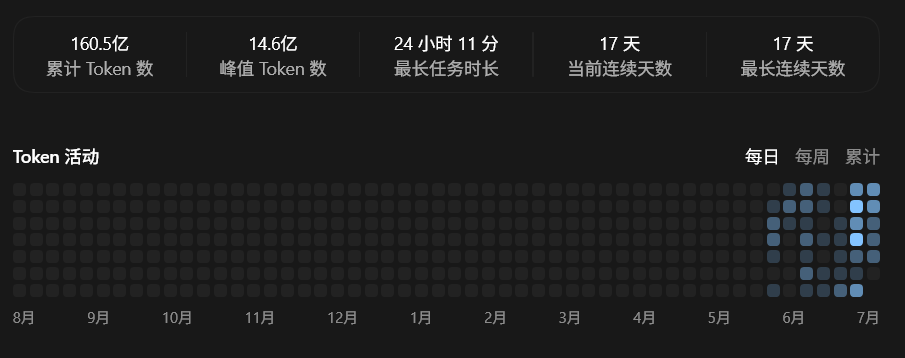
\includegraphics[width=0.78\linewidth]{token-activity.png}
  \caption{同期账户 Token 活动截图。累计 160.5 亿、峰值 14.6 亿、最长任务 24 小时 11 分、
  当前与最长连续天数均为 17 天。该图只说明使用规模和连续性，不证明工程质量、个人贡献、
  生产率或本文任何因果结论。}
  \label{fig:token-activity}
\end{figure}

\end{document}
